\documentclass[crop,tikz]{standalone}
\begin{document}
\usetikzlibrary{arrows}
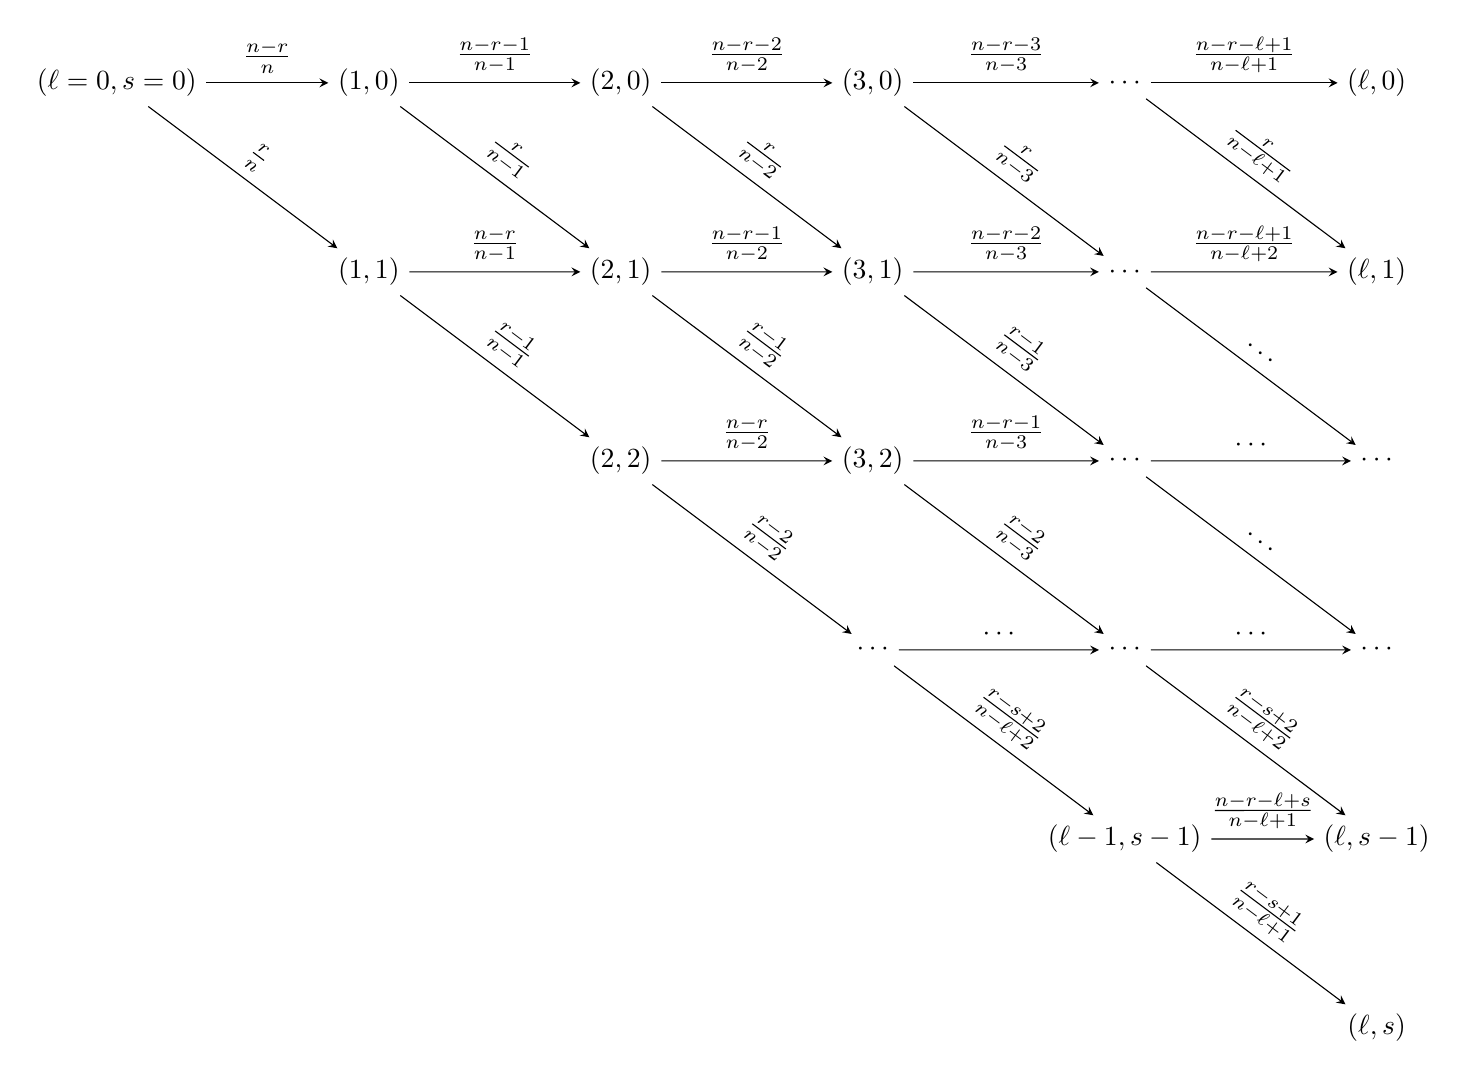
\begin{tikzpicture}[scale=3.2]
  \pgfmathsetmacro{\vh}{-0.75}
  \tikzstyle{coordinate}=[inner sep=0pt,outer sep=0pt]
  \tikzstyle{solid}=[color=black, thin, >=stealth]
  \tikzstyle{dots}=[color=black, thin, >=stealth]
  \node (P00) at (0,0*\vh) {$(\ell=0,s=0)$};
  \node (P10) at (1,0*\vh) {$(1,0)$};
  \node (P11) at (1,1*\vh) {$(1,1)$};
  \node (P20) at (2,0*\vh) {$(2,0)$};
  \node (P21) at (2,1*\vh) {$(2,1)$};
  \node (P22) at (2,2*\vh) {$(2,2)$};
  \node (P30) at (3,0*\vh) {$(3,0)$};
  \node (P31) at (3,1*\vh) {$(3,1)$};
  \node (P32) at (3,2*\vh) {$(3,2)$};
  \node (P33) at (3,3*\vh) {$\cdots$};
  \node (P40) at (4,0*\vh) {$\cdots$};
  \node (P41) at (4,1*\vh) {$\cdots$};
  \node (P42) at (4,2*\vh) {$\cdots$};
  \node (P43) at (4,3*\vh) {$\cdots$};
  \node (P44) at (4,4*\vh) {$(\ell-1,s-1)$};
  \node (P50) at (5,0*\vh) {$(\ell,0)$};
  \node (P51) at (5,1*\vh) {$(\ell,1)$};
  \node (P52) at (5,2*\vh) {$\cdots$};
  \node (P53) at (5,3*\vh) {$\cdots$};
  \node (P54) at (5,4*\vh) {$(\ell,s-1)$};
  \node (P55) at (5,5*\vh) {$(\ell,s)$};
  \draw [solid,->] (P00) -- (P10) node[midway,above,sloped] {$\frac{n-r}{n}$};
  \draw [solid,->] (P00) -- (P11) node[midway,above,sloped] {$\frac{r}{n}$};
  \draw [solid,->] (P10) -- (P20) node[midway,above,sloped] {$\frac{n-r-1}{n-1}$};
  \draw [solid,->] (P10) -- (P21) node[midway,above,sloped] {$\frac{r}{n-1}$};
  \draw [solid,->] (P11) -- (P21) node[midway,above,sloped] {$\frac{n-r}{n-1}$};
  \draw [solid,->] (P11) -- (P22) node[midway,above,sloped] {$\frac{r-1}{n-1}$};
  \draw [solid,->] (P20) -- (P30) node[midway,above,sloped] {$\frac{n-r-2}{n-2}$};
  \draw [solid,->] (P20) -- (P31) node[midway,above,sloped] {$\frac{r}{n-2}$};
  \draw [solid,->] (P21) -- (P31) node[midway,above,sloped] {$\frac{n-r-1}{n-2}$};
  \draw [solid,->] (P21) -- (P32) node[midway,above,sloped] {$\frac{r-1}{n-2}$};
  \draw [solid,->] (P22) -- (P32) node[midway,above,sloped] {$\frac{n-r}{n-2}$};
  \draw [dots,->]  (P22) -- (P33) node[midway,above,sloped] {$\frac{r-2}{n-2}$};
  \draw [dots,->]  (P30) -- (P40) node[midway,above,sloped] {$\frac{n-r-3}{n-3}$};
  \draw [dots,->]  (P30) -- (P41) node[midway,above,sloped] {$\frac{r}{n-3}$};
  \draw [dots,->]  (P31) -- (P41) node[midway,above,sloped] {$\frac{n-r-2}{n-3}$};
  \draw [dots,->]  (P31) -- (P42) node[midway,above,sloped] {$\frac{r-1}{n-3}$};
  \draw [dots,->]  (P32) -- (P42) node[midway,above,sloped] {$\frac{n-r-1}{n-3}$};
  \draw [dots,->]  (P32) -- (P43) node[midway,above,sloped] {$\frac{r-2}{n-3}$};
  \draw [dots,->]  (P33) -- (P43) node[midway,above,sloped] {$\cdots$};
  \draw [dots,->]  (P33) -- (P44) node[midway,above,sloped] {$\frac{r-s+2}{n-\ell+2}$};
  \draw [dots,->]  (P40) -- (P50) node[midway,above,sloped] {$\frac{n-r-\ell+1}{n-\ell+1}$};
  \draw [dots,->]  (P40) -- (P51) node[midway,above,sloped] {$\frac{r}{n-\ell+1}$};
  \draw [dots,->]  (P41) -- (P51) node[midway,above,sloped] {$\frac{n-r-\ell+1}{n-\ell+2}$};
  \draw [dots,->]  (P41) -- (P52) node[midway,above,sloped] {$\cdots$};
  \draw [dots,->]  (P42) -- (P52) node[midway,above,sloped] {$\cdots$};
  \draw [dots,->]  (P42) -- (P53) node[midway,above,sloped] {$\cdots$};
  \draw [dots,->]  (P43) -- (P53) node[midway,above,sloped] {$\cdots$};
  \draw [dots,->]  (P43) -- (P54) node[midway,above,sloped] {$\frac{r-s+2}{n-\ell+2}$};
  \draw [dots,->]  (P44) -- (P54) node[midway,above,sloped] {$\frac{n-r-\ell+s}{n-\ell+1}$};
  \draw [dots,->]  (P44) -- (P55) node[midway,above,sloped] {$\frac{r-s+1}{n-\ell+1}$};
\end{tikzpicture}
\end{document}
